% 2.4 պարագրաֆում անդրադարձ է կատարվել հարթ դեկարտյան արտադրյալներին: $k$-չափանի ցանցը՝ $G(n_{1},n_{2},\ldots,n_{k})$, $n_{i}\in \mathbb{N}$, շղթաների դեկարտյան արտադրյալն է՝ $P_{n_{1}}\square P_{n_{2}}\square\cdots\square P_{n_{k}}$: Գլանը՝ $C(n_{1},n_{2})$, շղթայի և ցիկլի՝ $P_{n_{1}}\square C_{n_{2}}$, իսկ k-չափանի տոռը՝ $T(n_{1},n_{2},\ldots,n_{k})$, ցիկլերի դեկարտյան արտադրյալն է՝ $C_{n_{1}}\square C_{n_{2}}\square\cdots\square C_{n_{k}}$:

\begin{frame}{Հարթ դեկարտյան արտադրյալներ}
\begin{columns}
\begin{column}{0.5\textwidth}
\begin{lemma}[Բեհզադ, Մահմուդիան, 1969] $G \square H$ դեկարտյան արտադրյալը հարթ է այն և միայն դեպքում, եթե
\begin{enumerate}
    \item<2-> $G\square H \cong P_m \square P_n$,
    \item<3-> $G\square H \cong C_m \square P_n$ կամ
    \item<4-> $G \cong K_2$, իսկ $H$-ը արտաքին հարթ գրաֆ է:
\end{enumerate}
\end{lemma}
\end{column}

\begin{column}{0.5\textwidth}
\only<2>{
    
    \begin{figure}[t!]
    \centering
    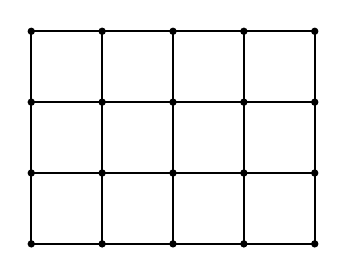
\begin{tikzpicture}[style=thick,scale=0.45, every node/.style={scale=0.45}]
        \coordinate (V11) at (2cm,2cm);
        \coordinate (V12) at (4cm,2cm);
        \coordinate (V13) at (6cm,2cm);
        \coordinate (V14) at (8cm,2cm);
        \coordinate (V15) at (10cm,2cm);
        \coordinate (V21) at (2cm,4cm);
        \coordinate (V22) at (4cm,4cm);
        \coordinate (V23) at (6cm,4cm);
        \coordinate (V24) at (8cm,4cm);
        \coordinate (V25) at (10cm,4cm);
        \coordinate (V31) at (2cm,6cm);
        \coordinate (V32) at (4cm,6cm);
        \coordinate (V33) at (6cm,6cm);
        \coordinate (V34) at (8cm,6cm);
        \coordinate (V35) at (10cm,6cm);
        \coordinate (V41) at (2cm,8cm);
        \coordinate (V42) at (4cm,8cm);
        \coordinate (V43) at (6cm,8cm);
        \coordinate (V44) at (8cm,8cm);
        \coordinate (V45) at (10cm,8cm);
        
        \draw (V11) -- (V12) -- (V13) -- (V14) -- (V15);
        \draw (V21) -- (V22) -- (V23) -- (V24) -- (V25);
        \draw (V31) -- (V32) -- (V33) -- (V34) -- (V35) ;
        \draw (V41) -- (V42) -- (V43) -- (V44) -- (V45) ;
        
        \draw (V11) -- (V21) -- (V31) -- (V41);
        \draw (V12) -- (V22) -- (V32) -- (V42);
        \draw (V13) -- (V23) -- (V33) -- (V43);
        \draw (V14) -- (V24) -- (V34) -- (V44);
        \draw (V15) -- (V25) -- (V35) -- (V45);
        
        \draw[fill=black] (V11) circle (2pt) ;
        \draw[fill=black] (V12) circle (2pt) ;
        \draw[fill=black] (V13) circle (2pt) ;
        \draw[fill=black] (V14) circle (2pt) ;
        \draw[fill=black] (V15) circle (2pt) ;
        \draw[fill=black] (V21) circle (2pt) ;
        \draw[fill=black] (V22) circle (2pt) ;
        \draw[fill=black] (V23) circle (2pt) ;
        \draw[fill=black] (V24) circle (2pt) ;
        \draw[fill=black] (V25) circle (2pt) ;
        \draw[fill=black] (V31) circle (2pt) ;
        \draw[fill=black] (V32) circle (2pt) ;
        \draw[fill=black] (V33) circle (2pt) ;
        \draw[fill=black] (V34) circle (2pt) ;
        \draw[fill=black] (V35) circle (2pt) ;
        \draw[fill=black] (V41) circle (2pt) ;
        \draw[fill=black] (V42) circle (2pt) ;
        \draw[fill=black] (V43) circle (2pt) ;
        \draw[fill=black] (V44) circle (2pt) ;
        \draw[fill=black] (V45) circle (2pt) ;
    \end{tikzpicture}
    \end{figure}
}
\only<3>{
 \begin{figure}[t!]
    \centering
    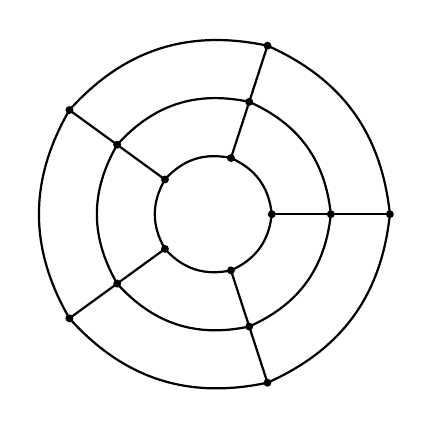
\begin{tikzpicture}[style=thick,scale=0.5, every node/.style={scale=0.5}]
        \coordinate (V11) at (0:1.5cm);
        \coordinate (V12) at (72:1.5cm);
        \coordinate (V13) at (144:1.5cm);
        \coordinate (V14) at (216:1.5cm);
        \coordinate (V15) at (288:1.5cm);
        \coordinate (V21) at (0:3cm);
        \coordinate (V22) at (72:3cm);
        \coordinate (V23) at (144:3cm);
        \coordinate (V24) at (216:3cm);
        \coordinate (V25) at (288:3cm);
        \coordinate (V31) at (0:4.5cm);
        \coordinate (V32) at (72:4.5cm);
        \coordinate (V33) at (144:4.5cm);
        \coordinate (V34) at (216:4.5cm);
        \coordinate (V35) at (288:4.5cm);
        
        
        \draw (V11) edge [bend right=30] (V12);
        \draw (V12) edge [bend right=30] (V13);
        \draw (V13) edge [bend right=30] (V14);
        \draw (V14) edge [bend right=30] (V15);
        \draw (V15) edge [bend right=30] (V11);
        \draw (V21) edge [bend right=30] (V22);
        \draw (V22) edge [bend right=30] (V23);
        \draw (V23) edge [bend right=30] (V24);
        \draw (V24) edge [bend right=30] (V25);
        \draw (V25) edge [bend right=30] (V21);
        \draw (V31) edge [bend right=30] (V32);
        \draw (V32) edge [bend right=30] (V33);
        \draw (V33) edge [bend right=30] (V34);
        \draw (V34) edge [bend right=30] (V35);
        \draw (V35) edge [bend right=30] (V31);
        
        
        \draw (V11) -- (V21) -- (V31) ;
        \draw (V12) -- (V22) -- (V32) ;
        \draw (V13) -- (V23) -- (V33) ;
        \draw (V14) -- (V24) -- (V34) ;
        \draw (V15) -- (V25) -- (V35) ;
        
        \draw[fill=black] (V11) circle (2pt) ;
        \draw[fill=black] (V12) circle (2pt) ;
        \draw[fill=black] (V13) circle (2pt) ;
        \draw[fill=black] (V14) circle (2pt) ;
        \draw[fill=black] (V15) circle (2pt) ;
        \draw[fill=black] (V21) circle (2pt) ;
        \draw[fill=black] (V22) circle (2pt) ;
        \draw[fill=black] (V23) circle (2pt) ;
        \draw[fill=black] (V24) circle (2pt) ;
        \draw[fill=black] (V25) circle (2pt) ;
        \draw[fill=black] (V31) circle (2pt) ;
        \draw[fill=black] (V32) circle (2pt) ;
        \draw[fill=black] (V33) circle (2pt) ;
        \draw[fill=black] (V34) circle (2pt) ;
        \draw[fill=black] (V35) circle (2pt) ;
    \end{tikzpicture}
    \end{figure}
}

\only<4>{
    \begin{figure}[t!]
    \centering
    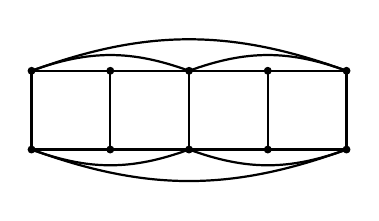
\begin{tikzpicture}[style=thick,scale=0.5, every node/.style={scale=0.5}]
        \coordinate (V11) at (2cm,2cm);
        \coordinate (V12) at (4cm,2cm);
        \coordinate (V13) at (6cm,2cm);
        \coordinate (V14) at (8cm,2cm);
        \coordinate (V15) at (10cm,2cm);
        \coordinate (V21) at (2cm,4cm);
        \coordinate (V22) at (4cm,4cm);
        \coordinate (V23) at (6cm,4cm);
        \coordinate (V24) at (8cm,4cm);
        \coordinate (V25) at (10cm,4cm);
        
        
        \draw (V21) edge [bend left=20] (V25);
        \draw (V21) edge [bend left=20] (V23);
        \draw (V23) edge [bend left=20] (V25);
        
        \draw (V11) edge [bend right=20] (V15);
        \draw (V11) edge [bend right=20] (V13);
        \draw (V13) edge [bend right=20] (V15);
        
        
        \draw (V11) -- (V12) -- (V13) -- (V14) -- (V15);
        \draw (V21) -- (V22) -- (V23) -- (V24) -- (V25);
        
        
        \draw (V11) -- (V21) ;
        \draw (V12) -- (V22) ;
        \draw (V13) -- (V23) ;
        \draw (V14) -- (V24) ;
        \draw (V15) -- (V25) ;
        
        \draw[fill=black] (V11) circle (2pt) ;
        \draw[fill=black] (V12) circle (2pt) ;
        \draw[fill=black] (V13) circle (2pt) ;
        \draw[fill=black] (V14) circle (2pt) ;
        \draw[fill=black] (V15) circle (2pt) ;
        \draw[fill=black] (V21) circle (2pt) ;
        \draw[fill=black] (V22) circle (2pt) ;
        \draw[fill=black] (V23) circle (2pt) ;
        \draw[fill=black] (V24) circle (2pt) ;
        \draw[fill=black] (V25) circle (2pt) ;
    \end{tikzpicture}
    \end{figure}
    
}
\end{column}
\end{columns}
\end{frame}

\begin{frame}[squeeze]{Հարթ դեկարտյան արտադրյալներ}
\begin{itemize}
\item Ուսումնասիրել են Գիառոն և Կուբալը (1997), Պետրոսյանը և Կարապետյանը (2007), Խչոյանը (2010):
\end{itemize}

\begin{columns}
\begin{column}{0.7\textwidth}

\begin{theorem}[2.4.6]
Եթե $m\geq 3, n\in \mathbb{N}$, ապա $P_m \square C_{2n+1} \in \mathfrak{N}$ և
\begin{center}
$w\left(P_m \square C_{2n+1}\right)= \left\{
\begin{tabular}{ll}
$4$, & երբ $m$-ը զույգ է,\\
$6$, & երբ $m$-ը կենտ է:\\
\end{tabular}%
\right.$
\end{center}
\end{theorem}

\begin{itemize}
\item Նաև ստացվել են $W(G)$ պարամետրի գնահատականներ, երբ $G = P_{n_{1}} \square P_{n_{2}} \square \ldots \square P_{n_k}$ և $G=P_m \square C_{n}$:
\end{itemize}
\end{column}

\begin{column}{0.3\textwidth}
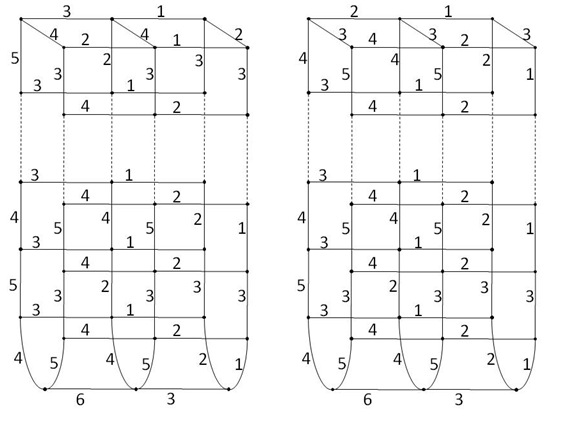
\includegraphics[width=\textwidth,trim={9cm 0 0 0},clip]{figures/cylinders.jpg}
\end{column}
\end{columns}

\begin{hide}
\begin{theorem}
\label{t2_planars} Եթե $G\square H$ դեկարտյան արտադրյալը հարթ է, ընդ որում 2 արտադրիչներն էլ ունեն առնվազն $3$ գագաթ, ապա $G\square H\in \mathfrak{N}$ և $w(G\square H)\leq 6$:
\end{theorem}
\end{hide}

\begin{hide}
\begin{theorem} Երբ $m\in\mathbb{N},n\geq 2$, 
\begin{center}
$W(C(2m,2n))\geq 4m+2n-2$,
\end{center}
իսկ երբ $m,n\in\mathbb{N}$,
\begin{center}
$W(C(2m,2n+1))\geq 4m+2n-1$:
\end{center}
\end{theorem}
\end{hide}

\end{frame}

\begin{frame}[shrink]{Դեֆիցիտ}
\begin{columns}
\begin{column}{0.6\textwidth}<2->

Եթե $\alpha$-ն $G$-ի ճիշտ կողային ներկում է, ապա
\begin{itemize}
\item $def(v, \alpha)=\overline{S}(v,\alpha) - \underline{S}(v,\alpha) - |S(v,\alpha)| + 1$,
\item $def(G, \alpha) = \sum\limits_{v \in V(G)}{def(v,\alpha)}$,
\item $def(G) = \min\limits_{\alpha}{def(G,\alpha)}$, որտեղ մինիմումը վերցվում է ըստ $G$-ի բոլոր ճիշտ ներկումների,
\end{itemize}
\end{column}
\begin{column}{0.4\textwidth}
\begin{figure}
  \begin{center}
  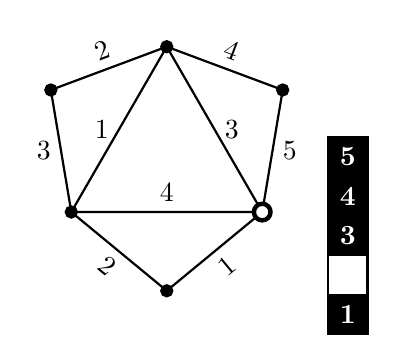
\begin{tikzpicture}[style=thick]
    \draw (90:1.4cm) -- node [right] {$3$}  
    (-30:1.4cm) -- node [sloped,above] {$4$} 
    (-150:1.4cm) -- node [left] {$1$} cycle;
    \draw (90:1.4cm) -- node [sloped,above] {$2$}  
    (150:1.7cm) -- node [left] {$3$}  
    (-150:1.4cm) -- node [sloped,below] {$2$}  
    (-90:1.7cm) -- node [sloped,below] {$1$}  
    (-30:1.4cm) -- node [right] {$5$} 
    (30:1.7cm) -- node [sloped,above] {$4$} cycle;
    
    \draw[fill=black] (90:1.4cm) circle (2pt);
    \draw[fill=white,style=ultra thick] (-30:1.4cm) circle (3pt);
    \draw[fill=black] (-150:1.4cm) circle (2pt);
    \draw[fill=black] (150:1.7cm) circle (2pt);
    \draw[fill=black] (-90:1.7cm) circle (2pt);
    \draw[fill=black] (30:1.7cm) circle (2pt);
    
    \node[draw,fill=black,text=white,minimum height=0.5cm,minimum width=0.5cm] at (2.3cm,-2cm) {$\mathbf{1}$};
    \node[draw,fill=white,text=white,minimum height=0.5cm,minimum width=0.5cm] at (2.3cm,-1.5cm) {$\mathbf{2}$};
    \node[draw,fill=black,text=white,minimum height=0.5cm,minimum width=0.5cm] at (2.3cm,-1cm) {$\mathbf{3}$};
    \node[draw,fill=black,text=white,minimum height=0.5cm,minimum width=0.5cm] at (2.3cm,-0.5cm) {$\mathbf{4}$};
    \node[draw,fill=black,text=white,minimum height=0.5cm,minimum width=0.5cm] at (2.3cm,0cm) {$\mathbf{5}$};
  \end{tikzpicture}
  \end{center}
\end{figure}

\end{column}
\end{columns}
\end{frame}

\begin{frame}[shrink]{Անցքերի թիվ}
\begin{columns}
\begin{column}{0.6\textwidth}

Եթե $\alpha$-ն $G$-ի ճիշտ կողային ներկում է, ապա
\begin{itemize}
\item $gn(G, \alpha) = \max\limits_{v \in V(G)}{def(v,\alpha)}$,
\item $gn(G) = \min\limits_{\alpha}{gn(G,\alpha)}$, որտեղ մինիմումը վերցվում է ըստ $G$-ի բոլոր ճիշտ կողային ներկումների,
\item $gn(G) \leq def(G) \leq gn(G)|V(G)|$:
\end{itemize}
\end{column}

\begin{column}{0.4\textwidth}
\begin{figure}
  \begin{center}
  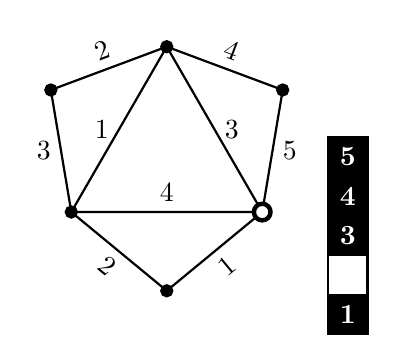
\begin{tikzpicture}[style=thick]
    \draw (90:1.4cm) -- node [right] {$3$}  
    (-30:1.4cm) -- node [sloped,above] {$4$} 
    (-150:1.4cm) -- node [left] {$1$} cycle;
    \draw (90:1.4cm) -- node [sloped,above] {$2$}  
    (150:1.7cm) -- node [left] {$3$}  
    (-150:1.4cm) -- node [sloped,below] {$2$}  
    (-90:1.7cm) -- node [sloped,below] {$1$}  
    (-30:1.4cm) -- node [right] {$5$} 
    (30:1.7cm) -- node [sloped,above] {$4$} cycle;
    
    \draw[fill=black] (90:1.4cm) circle (2pt);
    \draw[fill=white,style=ultra thick] (-30:1.4cm) circle (3pt);
    \draw[fill=black] (-150:1.4cm) circle (2pt);
    \draw[fill=black] (150:1.7cm) circle (2pt);
    \draw[fill=black] (-90:1.7cm) circle (2pt);
    \draw[fill=black] (30:1.7cm) circle (2pt);
    
    \node[draw,fill=black,text=white,minimum height=0.5cm,minimum width=0.5cm] at (2.3cm,-2cm) {$\mathbf{1}$};
    \node[draw,fill=white,text=white,minimum height=0.5cm,minimum width=0.5cm] at (2.3cm,-1.5cm) {$\mathbf{2}$};
    \node[draw,fill=black,text=white,minimum height=0.5cm,minimum width=0.5cm] at (2.3cm,-1cm) {$\mathbf{3}$};
    \node[draw,fill=black,text=white,minimum height=0.5cm,minimum width=0.5cm] at (2.3cm,-0.5cm) {$\mathbf{4}$};
    \node[draw,fill=black,text=white,minimum height=0.5cm,minimum width=0.5cm] at (2.3cm,0cm) {$\mathbf{5}$};
  \end{tikzpicture}
  \end{center}
\end{figure}
\end{column}
\end{columns}
\end{frame}

\begin{frame}{Գրաֆների դեֆիցիտի մասին հիպոթեզ}
\begin{theorem}[Գիառո, Կուբալ, Մալաֆիյսկի, 1999]
Գոյություն ունի գրաֆների $\left\{G_n\right\}$ հաջորդականություն այնպես, որ $\lim_{n \rightarrow \infty}{\frac{def(G_n)}{|V(G_n)|}} = 1$:
\end{theorem}

\begin{hypothesis}
Ցանկացած $G$ գրաֆի համար $def(G) \leq |V(G)|$:
\end{hypothesis}
\end{frame}


\begin{frame}[shrink]{Արտաքին հարթ գրաֆների դեֆիցիտ}
$f_i(G)$-ն $G$ արտաքին հարթ գրաֆում $i$ կողեր ունեցող վերջավոր նիստերի քանակն է, որտեղ $i=3,4,\ldots,|V(G)|$:

\begin{theorem}[2.4.15]
Եթե $G$-ն արտաքին հարթ գրաֆ է, ապա 
\begin{center}
$def(G) \leq \sum\limits_{\substack{i\geq 3 \\ \text{կենտ }i}}{f_i(G)}$ և $gn(G) \leq f_3(G) + \min\{1,  \sum\limits_{\substack{i\geq 5 \\ \text{կենտ }i}}{f_{i}(G)} \}$
\end{center}
\end{theorem}

\begin{itemize}
\item Ընդհանրացնում է երկկողմանի արտաքին հարթ գրաֆների մասին Գիառոյի և Կուբալի արդյունքը (2004):
\end{itemize}

\end{frame}


\begin{frame}[shrink]{Արտաքին հարթ գրաֆների դեֆիցիտ}


\begin{corollary}[2.4.17]
Եթե $G$-ն եռանկյուն չպարունակող արտաքին հարթ գրաֆ է, ապա $gn(G) \leq 1$: 
\end{corollary}

\begin{corollary}[2.4.18]
Եթե $G$-ն արտաքին հարթ գրաֆ է, ապա 
$def(G) \leq \frac{|V(G)|-2}{og(G)-2} \leq |V(G)|$,
որտեղ $og(G)$-ն $G$-ի կարճագույն կենտ ցիկլի երկարությունն է:
\end{corollary}
\end{frame}